Although process mining in the business domain is a well-established field with 
much software developed up to date (ERP, WFM and other systems), 
``Business Process Intelligence'' tools usually do not perform process discovery
and typically offer relatively simple analyzes that depend upon a correct
a-priori process model \cite{citeulike:3718014} \cite{citeulike:5044991}.
Moreover, they heavily depend on well composed and annotated process logs as
required by process mining manifesto \cite{citeulike:11077707}:
``All process mining techniques assume that it is possible to sequentially 
record events such that each event refers to an activity (i.e., a well-defined 
step in some process) and is related to a particular case (i.e., a process instance).''

This facts restricts direct application of business domain process mining techniques
to software engineering, where processes are usually performed concurrently by
many agents, are more complex and typically have a higher level of noise. Taking
this fact in account, I will review only the approaches to the mining for which
applicability to software process mining was expressed. 

A set of findings relevant to my research approach was developed by Rubin
et al. \cite{citeulike:1885717} and van der Aalst et al.
\cite{citeulike:3718014} and is called \textit{incremental workflow mining}. The
authors not only designed sophisticated algorithms but built a software system
using a business process mining framework called ProM by van Dongen et al.
\cite{citeulike:5043673} which synthesizes a Petri Net corresponding to the
observed process. The system was tested on SCM logs and while the process
artifacts retrieved from the SCM system are rather high-level, the approach
discussed is very promising for the modeling of software processes from the
low-level product and process data.

\begin{figure}[tbp]
   \centering
   \includegraphics[height=65mm]{petri-log.eps}
   \caption{Illustration of the required log pre-processing step step 
before BPI tools application from \cite{citeulike:1885717}. During this step,
the development log is annotated manually.}
   \label{fig:petri-log}
\end{figure}

\begin{figure}[tbp]
   \centering
   \includegraphics[height=65mm]{petri.eps}
   \caption{Illustration of the ``Generation and Synthesis Approach'' from
\cite{citeulike:5043673}: a) Transition System with regions shown; b),c) Petri
Nets synthesized from the Transition System.}
   \label{fig:petri}
\end{figure}

Within the incremental workflow mining framework, the input data from the SCM
audit trail information is mapped to the event chain which corresponds to the
software process artifacts. The authors call this process \textit{abstraction on
the log level} which is implemented as a set of filters which not only
aggregates basic events into single high-level entities but also removes data
irrelevant to the mining process (noise). 

The event chain constructed through the abstraction is then treated with the
\textit{Generate} part of the \textit{``Generate and Synthesis''}
\cite{citeulike:3718014} algorithm in order to generate a \textit{Transition
System} which represents an ordered series of events. This algorithm looks at
the history (prefix) and the future (suffix) sequences of events related to the
current one in order to discover transitions.  When applied to the abstracted
log information, the algorithm generates a rather large Transition System graph
where edges connect to abstracted events. This transition system is then
successively simplified by using various reduction strategies such as ``Kill
Loops'', ``Extend'', ``Merge by Output'' and others; it is possible to combine
these reduction strategies in order to achieve a greater simplification.

At the last step of the incremental workflow mining approach, Transition Systems
are used to \textit{Synthesize} labeled Petri nets (where different transition
can refer to the same event) with the help of \textit{``regions theory''}
\cite{citeulike:5128170}. As with the Transition System generation, the authors
investigate many different strategies of Petri nets synthesis, showing
significant variability in the results achieved. (see Figure \ref{fig:petri}).

The significant contribution of this research is in the generality of the
method. It was shown that by tuning the ``Generate'' and ``Synthesize'' phases
it is possible to tailor the algorithm to a wide variety of processes. In
particular, as mentioned before, Rubin et al. successfully applied this
framework to the SCM logs analysis.